\documentclass{emulateapj}
% DSS: Test worked.

% To do 
% 1) consistency between p and P for pressure
% 2) Signs in fluxes... and overall consistency (is Fint everywhere it
%    needs to be?)

% GSN test add 2

% To do when things have stabalized a bit
% 1) Define all terms
% 2) acronyms

% DSS comments
% 1) Where do the 2's, 3's, pi's come from...?
% 2) A lot of material feels like appendix material

% Response to DSS comments
% 1) Will get defns, etc, on first use when paper is further along.
% 2) Should the appendix material be there at all?  That's the decision.

% GSN test add

\usepackage{epsfig}
\usepackage{amsmath}
\usepackage{rotating}
\usepackage{natbib}
% \usepackage{lscape}
\usepackage{enumerate}
\usepackage{multirow}
\usepackage{array}
\usepackage{appendix}
\usepackage{comment}

\bibliographystyle{apj}
\defcitealias{robinson+catling2012}{RC}

\def\plotonesc#1{\centering \leavevmode
\includegraphics[clip=, width=1.70\columnwidth]{#1}}
\def\plotoneh#1{\centering \leavevmode
\includegraphics[clip=, width=.95\columnwidth]{#1}}
\def\plotone#1{\centering \leavevmode
\includegraphics[clip=, width=.85\columnwidth]{#1}}
\def\plotoneShrinkSmall#1{\centering \leavevmode
\includegraphics[clip=, width=.49\columnwidth]{#1}}
\def\plotoneShrinkMed#1{\centering \leavevmode
\includegraphics[clip=, width=.55\columnwidth]{#1}}
\def\plotoneShrinkBig#1{\centering \leavevmode
\includegraphics[clip=, width=.65\columnwidth]{#1}}
\def\plottwo#1#2{\centering \leavevmode
\includegraphics[width=.45\columnwidth]{#1} \hfil
\includegraphics[width=.45\columnwidth]{#2}}
\def\plottwob#1#2{\centering \leavevmode
\includegraphics[width=.49\columnwidth]{#1} \hfil
\includegraphics[width=.49\columnwidth]{#2}}
\def\plottwor#1#2{\centering \leavevmode
\includegraphics[width=.55\columnwidth,angle=90]{#1} \hfil
\includegraphics[width=.55\columnwidth,angle=90]{#2}}
\def\plotthree#1#2#3{\centering \leavevmode
\includegraphics[width=.3\columnwidth]{#1} \hfil
\includegraphics[width=.3\columnwidth]{#2} \hfil
\includegraphics[width=.3\columnwidth]{#3}}

% notation that's likely to change
\newcommand{\fsum}{F_I}
\newcommand{\fshc}{F_{I,HC}}
\newcommand{\sigmasb}{\sigma_{\rm SB}}
\newcommand{\compton}{\bar{\lambda}}
\newcommand{\nablaAd}{\nabla_{\rm ad}}
\newcommand{\nablaRad}{\nabla_{\rm rad}}
\newcommand{\scale}[2]{\left(\frac{#1}{#2}\right)}
\newcommand{\unit}[1]{\,\hbox{#1}}

\newcommand{\cN}[1]{\mathcal{N}}
\newcommand{\pn}[1]{\mbox{$(#1)$}}
\newcommand{\spa}{\mbox{ }}
\def\gsim{\;\rlap{\lower 2.5pt
 \hbox{$\sim$}}\raise 1.5pt\hbox{$>$}\;}
\def\lsim{\;\rlap{\lower 2.5pt
   \hbox{$\sim$}}\raise 1.5pt\hbox{$<$}\;}

% set formatting properties
\setlength{\textwidth}{6.5in}
\setlength{\textheight}{9in}
\setlength{\hoffset}{0.in}
\setlength{\voffset}{-0.5in}
%\setlength{\voffset}{0.3in}
\parindent 0.2in
\parskip 0.1in



%%%%%%%%%%%%%%%%%%%%%%%%%%%%%%%%%%%%%%%%%%%%%%%%%
% THE DOCUMENT BEGINS HERE                      %
%%%%%%%%%%%%%%%%%%%%%%%%%%%%%%%%%%%%%%%%%%%%%%%%%

%\slugcomment{Submitted to ApJ, 20 October 2011}

\begin{document}


%%% Begin front material
%\twocolumn[%%% Begin front material

\title{Planet Evolution}


\author{
%
Greg Novak\altaffilmark{1},
%
David S. Spiegel\altaffilmark{2}
}

\affil{$^1$IAP}

\affil{$^2$Astrophysics Department, Institute for Advanced Study,
  Princeton, NJ 08540}


\vspace{0.5\baselineskip}

\email{
greg.novak@obspm.fr,
dave@ias.edu
}


\begin{abstract}
This is an abstract
\end{abstract}


\keywords{planetary systems -- radiative transfer}
%]%%% End front material

\section{Introduction}
\label{sec:intro}
One of the goals of this work is to present the community with an
easy-to-use, publicly available, robust platform for experimentation
with planet evolution.

Another goal is to provide the simplest complete model for planet
evolution that includes a ideal gas EOS, a degenerate gas EOS, and an
atmosphere model.  This is for pedagogical purposes as well as to
facilitate mapping of the large parameter space without running a
``full blown'' simulation, which potentially includes many free
parameters that are very poorly constrained (such as the exact
abundances of each element).  

\section{Middle}

\label{sec:mid}

\subsection{Equation of State}

\subsubsection{Gas Phase}
% FIXME -- check equations in this section against some reference for
% having the right constants in front.
Roughly copy useful text and equations out of my own notes.  Wish that
I hadn't formulated anything in terms of sound speed.  Should have
just used energy.  Will need to change this.

It is easy to write down an equation of state that covers all major
regimes of the gas-phase equation of state: ideal gas,
non-relativistic degenerate gas, relativistic degenerate gas,
relativistic non-degenerate gas.

Basic changes in the physics occur when the Fermi energy and thermal
energies are equal; when the Fermi velocity approaches $c$; and when
the thermal velocity approaches $c$.  

Relativistic effects become important when the thermal energy is
greater than the rest mass energy
\begin{equation}
k T > \frac{2}{3} m_e c^2
\end{equation}
for electrons, and similarly for protons.

The Fermi momentum for spin 1/2 particles is
\begin{equation}
  % Landau + Lifshitz Statistical Physics 3rd ed eq 57.2 p 166
  p_F = (3 \pi^2)^{1/3} Y_e^{1/3} n_b^{1/3} \hbar
\end{equation}
where $Y_e$ is the number of electrons per baryon:
\begin{equation}
  Y_e = \frac{n_e}{n_b}
\end{equation}
Then the Fermi energy is $E_F = p_F^2/2 m$ if $E_f \ll m c^2$ and $E_F
= p_F c $ if $E_F \gg mc^2$. 

Degeneracy effects become important when the Fermi energy is equal to
the thermal energy, $3 k T / 2$.  Using the non-relativistic
expression for the Fermi energy
\begin{equation}
  k T = \frac{\pi^{4/3} \hbar c Y_e^{2/3} n_b^{2/3} \compton_e}{3^{1/3}}
% FIXME -- changed condition here, check code
% 2\pi\hbar c Y_e^{2/3} n_b^{2/3} \bar{\lambda}_e
\end{equation}
while for protons it is 
\begin{equation}
  k T = \frac{\pi^{4/3} \hbar c n_b^{2/3} \compton_p}{3^{1/3}}
\end{equation}

Using the relativistic expression for the Fermi energy yields
\begin{equation}
  \frac{2 \pi^{2/3}}{3^{2/3}} \hbar c Y_e^{1/3} n_b^{1/3}
\end{equation}
for electrons and 
\begin{equation}
  \frac{2 \pi^{2/3}}{3^{2/3}} \hbar c n_b^{1/3}
\end{equation}
for protons.

The relevant physics also changes when the Fermi energy becomes larger
than the rest mass energy of the particles:
\begin{equation}
  % FIXME -- this changed: check code
  n_b = \frac{2^{3/2} \compton_e^{-3}}{3 \pi^2 Y_e}
  % old value: \left(\frac{2^{3/2}}{3^{1/3} \pi^{2/3}}\right)  \compton_e^{-3} 
\end{equation}
and, for protons
\begin{equation}
  n_b = \frac{2^{3/2} \compton_p^{-3}}{3 \pi^2}
\end{equation}

\begin{figure*}
  \centering
  % from regime_plot() in ./gsn.py
  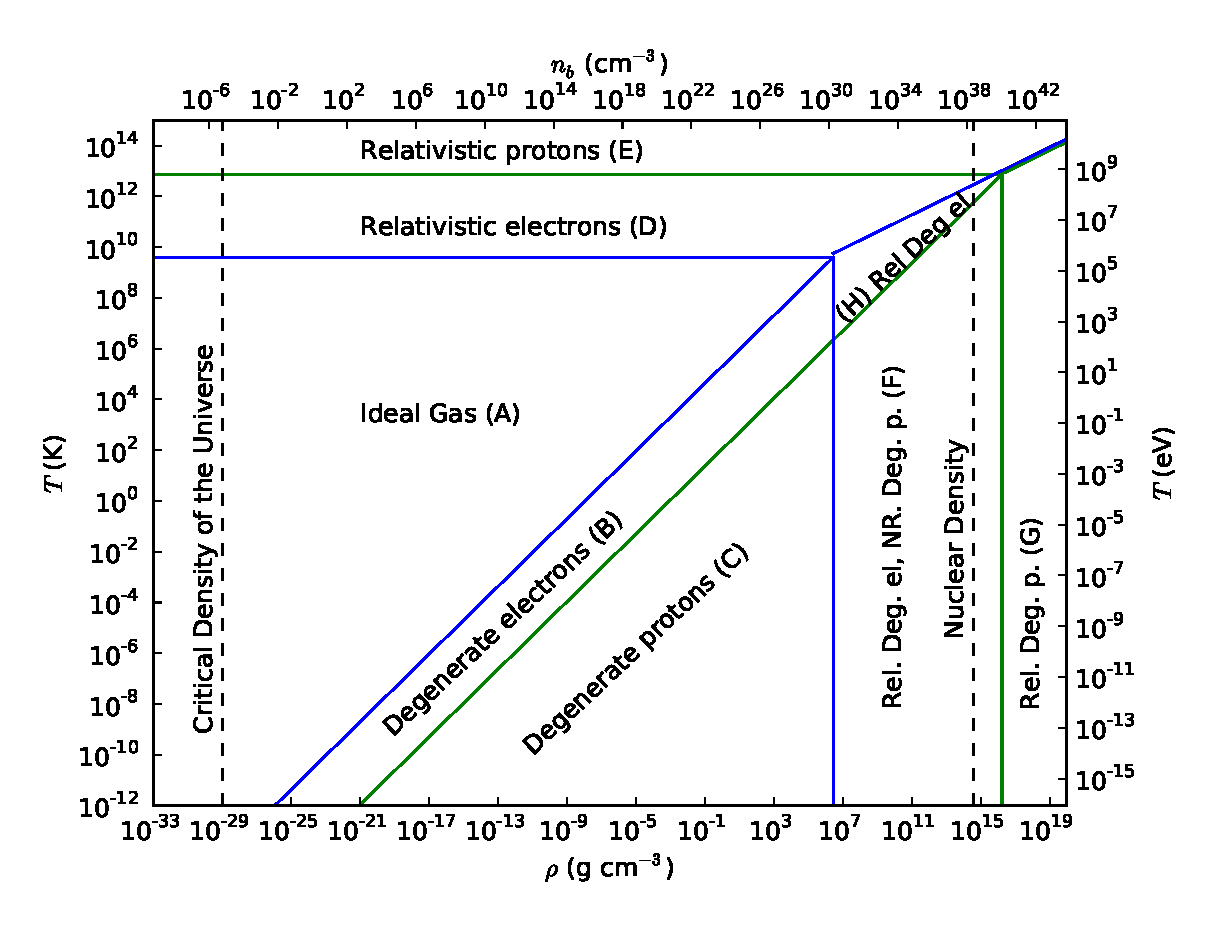
\includegraphics[width=0.9\textwidth]{f3}\\
  \caption{Phase diagram of the relevant regimes.  {\it Top:} The
    sound speeds given just use the non-relativistic idea gas formula.
    There are no relativistic corrections (so it can be greater than
    $c$), I don't worry about the how the mean molecular weight
    changes with temperature, or about how the sound speed changes
    when, e.g. the electrons are degenerate. {\it Bottom:} The dashed
    lines are just reference points and do not divide physical
    regions.}
  \label{fig:eos-regimes}
\end{figure*}

%\begin{figure*}
%  \centering
%  \caption{Here's a plot with the different regions just labeled for
%    reference later on.    This should be combined with
%    the previous fig.}
%\end{figure*}

For a single species, the expressions for pressure are:
$E_F < E_T < E_R$, (ND, NR ideal gas)
\begin{equation}
  p = n k T
\end{equation}
$E_T < E_F < E_R$, (D, NR gas of spin-2 fermions)
\begin{equation}
  p = \frac{(3 \pi^2)^{2/3}}{5} \frac{\hbar^2}{m} n^{5/3}
  % Landau + Lifshitz Statistical Physics 3rd ed eq 57.7 p 167
\end{equation}
$E_T < E_R < E_F$, or $E_R < E_T < E_F$ (D, R gas of spin-2 fermions)
\begin{equation}
  p = \frac{(3\pi^2)^{1/3}}{4} \hbar c n^{4/3}
  % Landau + Lifshitz Statistical Physics 3rd ed eq 61.4 p 178
\end{equation}
$E_F < E_R < E_T$ or $E_R < E_F < E_T$ (ND, R gas, $g=2$ bosons)
\begin{equation}
  p = \frac{\pi^2}{45} \frac{1}{\hbar^3 c^3} (kT)^4
% Kolb + Turner Section 3.3, page 62, eq 3.62  
\end{equation}
or, for fermions in the same limit:
\begin{equation}
  p = \frac{7}{8} p_{\rm Boson}
% Kolb + Turner Section 3.3, page 62, eq 3.62  
\end{equation}

Now the entropy is:
$E_F < E_T < E_R$, (ND, NR ideal gas)
\begin{equation}
  % Dimensionless entropy
  % Kittel + Kroemer Second ed. Chapter 3, eq 76, page 77
  \frac{\Sigma}{N} = \log\scale{n_Q}{n} + \frac{5}{2}
\end{equation}
with
\begin{equation}
  n_Q = \scale{m k T}{2\pi \hbar^2}^{3/2}
  % Kittel + Kroemer Second ed. Chapter 3, eq 63, page 73
\end{equation}
$E_T < E_F < E_R$, (D, NR gas of spin-2 fermions)
\begin{equation}
 \frac{\Sigma}{N} = \scale{\pi}{3}^{2/3} \frac{m}{\hbar^2} \frac{k T}{n^{2/3}}
  % Landau + Lifshitz Statistical Physics 3rd ed eq 58.5, 58.4 p 171
  % Note L+L use S = dimensionless entropy and T = temperature
  % measured in energy units, same as K+K
\end{equation}
$E_T < E_R < E_F$, or $E_R < E_T < E_F$ (D, R gas of spin-2 fermions)
\begin{equation}
  % Landau + Lifshitz Statistical Physics 3rd ed Section 61, Problem 2
  % solution, page 179
  \frac{\Sigma}{N} = \frac{\pi^{4/3}}{3^{1/3}} 
  \frac{1}{\hbar c}
  \frac{k T}{n^{1/3}}
  % The relation between E_T and E_R doesn't matter here because the
  % states that would normally open up when E_T > E_R (hence giving a
  % huge increase in entropy) are already full b/c E_F is above both
  % of them.
\end{equation}
$E_F < E_R < E_T$ or $E_R < E_F < E_T$ (ND, R gas, $g=2$ bosons)
\begin{equation}
  % Kolb + Turner Section 3.4, page 67, eq 3.72
  % using their non-dimensionalized entropy with hbar = c = k = 1
  % Their formula entropy per volume, not per baryon
  \frac{\Sigma}{N}  = \frac{4 \pi^2}{45} \frac{1}{\hbar^3 c^3} \frac{(kT)^3}{n} 
\end{equation}
or, for fermions in the same limit:
\begin{equation}
  % Kolb + Turner Section 3.4, page 67, eq 3.72
  % using their non-dimensionalized entropy with hbar = c = k = 1
  % Their formula gives entropy per volume, not per baryon
  s = \frac{7}{8} s_{\rm Boson}
  % The relation between E_F and E_R doesn't matter here because the
  % thermal energy is already high enough to lift degeneracy,
  % regardless of the fact that the Fermi energy _would_ be high
  % enough to have a relativistic degenerate gas _if_ the thermal
  % energy were lower.
\end{equation}
Finally, Kittel + Kroemer give the relation between their
dimensionless entropy and the ``conventional entropy.''  Landau +
Lifshitz use the same convention as Kittel + Kroemer, where
temperature is measured in energy and entropy is dimensionless.
\begin{equation}
  % Kittel + Kroemer, 2nd ed, Chapt 2, Eq 30, Page 43
  S = k \sigma
\end{equation}

Considering each region of \ref{fig:eos-regimes} in turn, for the
pressure we have the following.

%%% FIXME -- bookmark in verifying EOS equations

In region A
\begin{equation}
  p = n_b k T (1+X)
\end{equation}

In region B electrons are degenerate but protons are not.  The
condition for the protons to provide as much pressure is almost the
same as the condition for the electrons to be degenerate, so as you
become fully degenerate the protons become negligible.  So neglect
them in region B.  In region C, both electrons and protons are
degenerate, but the $m_p$ or $m_e$ that appears in the denominator
ensures that the proton contribution is always negligible.  In region
F, electrons are degenerate and relativistic while protons are
degenerate and non-relativistic.  The condition for the protons to
contribute is the same as for the proton Fermi energy to be such that
the protons are relativistic.  Therefore the protons are negligible in
region F.  Finally, in regions B, C, and F, the pressure is given by
degenerate electrons.
\begin{equation}
  p = \frac{ 3^{2/3} \pi^{4/3}}{40} \frac{\hbar^2 n_b^{5/3}}{m_e}
\end{equation}

In region G, both electrons and protons are degenerate and
relativistic.  The expression doesn't contain their rest mass so they
both contribute equally and you pick up a factor of 2.
\begin{equation}
  p = \frac{3^{4/3} \pi^{2/3} }{4} \hbar c n_b^{4/3}
\end{equation}

In region D protons are an ideal gas but the electrons are behaving
like photons, except for a factor of 7/8 due to Fermi statistics instead of
Bose-Einstein statistics.  
% See Kolb + Turner Section 3.3, page 60, eq 3.62, noting that rho
% refers to the total energy density, not the rest mass density
The condition for the protons to contribute is $n_b >
(\pi^2/45) (k T / \hbar c)^3$ (there must be more than one baryon per
mean photon wavelength), which falls in region H, so protons never
contribute.  Therefore in region D we have
\begin{equation}
  p = \frac{\pi^2 k^4 T^4}{45 c^3 \hbar^3}
\end{equation}

In region E, both protons and electrons are behaving like photons
\begin{equation}
  p = \frac{\Gamma \pi^2 k^4 T^4}{51 c^3 \hbar^3}
\end{equation}
where $\Gamma$ refers to the number of degrees of freedom (I think
this usage is standard) and is somewhere between 10 and a hundred.  In
region $I$, the same thing is going on but the electron states are
full, so it's the same expression with a value of $\Gamma$ decremented
by one.

In region H, the protons are behaving as an ideal gas while the
electrons are relativistic and degenerate.  The condition for the
baryons to contribute is almost the same as that given in the previous
paragraph, so for most/all of region H, the baryons dominate the
pressure.  Then we have:
\begin{equation}
  p = n_b k T 
\end{equation}

The reason that in the absence of cooling the equation of state is
proportional to $\rho^{5/3}$ in both the low density (adiabatic ideal
gas) and high density (degenerate fermion gas) state is that both
gases are dominated by the kinetic energy of the constituent
particles, while the potential energies associated with inter-particle
forces are negligible. \citep[][\S 57, p
168]{landau+lifshitz_statistical_physics_part_1}.  At intermediate
densities the interaction energies become comparable to the thermal
energies, the situation is much more complicated.  This happens to be
the situation at typical densities encountered in everyday life.

Comparing to the detailed equation of state given by... (Mesa?  Who?),
the pressures given in this section are accurate to... (a factor of
two?) over an enormous range of densities and temperatures.

Finally, consider the entropy in each of the regions given by Figure
\ref{fig:eos-regimes}.  

In region A, both electrons and protons are nonrelativisitc, so their
individual contributions to the entropy are given by the Sakur-Tetrode
equation: 

\begin{eqnarray}
\frac{\Sigma}{N_b} = \log \frac{n_q}{n}
  \label{eq:sakur-tetrode}
\end{eqnarray}
where 
\begin{equation}
  % Kittel + Kroemer 2nd ed Ch 3 eq 63 page 73
  n_q = \left(\frac{m_p kT}{2\pi\hbar^2}\right)^{3/2}
\end{equation}
is the density where degeneracy effects become important, the quantum
concentration.  It is the same as the condition we have already used
(thermal energy equal to the Fermi energy), up to a factor of order
unity.  The difference in definitiions is for convenience in writing
the Sakur-Tetrode equation.

Taking the Sakur-Tetrode equation for the protons and electrons plus
the entropy of mixing gives the total entropy, which is dominated by
the protons.
\begin{eqnarray}
\frac{\Sigma}{N_b} &=& (1+ X) \log\frac{n_{qe}}{n_b} + 
- (1-X)\log(1-X)  \nonumber \\
& & - 2 X \log X + X \frac{5}{2} 
+ \frac{3}{2} (\log\frac{m_p}{m_e} + \frac{5}{3}) 
\end{eqnarray}
In region B, the electron contribution switches to $(n_q/n)^{2/3}$ so
it's less than one and we have
\begin{equation}
\frac{\Sigma}{N_b} = \log\frac{n_{qe}}{n_b} 
- (1-X)\log(1-X) - X \log X 
+ \frac{3}{2} (\log\frac{m_p}{m_e} + \frac{5}{3})
\end{equation}
In region C, the proton contribution switches to the degenerate case.
In region F, the electrons are already negligible, so it doesn't
matter if they become relativistic.  In region G, it's not clear to me
if it matters that the Fermi sea of protons is becoming relativistic.
The entropy will be bounded above by one, but the expression may or
may not change.  Therefore in regions C, F, and maybe G, we have:
\begin{equation}
  \frac{\Sigma}{N_b} = \frac{2 \pi^{5/3}}{3^{2/3}}\left(\frac{n_{qp}}{n_b}\right)^{2/3}
\end{equation}
In region D, the entropy per baryon provided by the electrons is of
order the ratio of the photon density to the baryon density.
Temperatures are so high in this region that this will generally be
strongly dominated by the electrons.  Thus in region D the entropy per
baryon is
\begin{equation}
  \Sigma = \frac{4 \pi^2 \Gamma k^3 T^3}{45 \hbar^3 c^3 n_b}
  \label{eq:relativistic-entropy}
\end{equation}

Note that this is a bit confusing: When you have a mixture of high
mass and low mass non-relativistic particles, the massive particles
carry the entropy.  However, if you let the mass of the lower-mass
particle go to zero, then {\em it} carries the entropy.  Letting the
mass go to zero ensures that the particle becomes relativistic.  In
the {\em classical} expression for entropy (equation
\ref{eq:sakur-tetrode}), letting the mass go to zero makes the
quantum concentration zero, so there's no classical regime---it's
always quantum.  One would then conclude that gases of low-mass
particles have very little entropy.  However, the {\em relativistic}
expression (equation \ref{eq:relativistic-entropy}) gives large
entropy.  So it must be that passing to the relativistic limit is what
changes things so dramatically.  This bears further thought.

In region E, similar considerations to the previous section lead us to
the same expression for photons, with an additional factor for the
number of degrees of freedom being excited.  In region I, the same
thing is going on with one or two fewer degrees of freedom.  
\begin{equation}
  \Sigma = \frac{4 \pi^2 \Gamma k^3 T^3 V}{45 \hbar^3 c^3}
\end{equation}

In region H, the electrons are supposed to be degenerate so they
shouldn't contribute much entropy.  I suppose then that we're back to
the Sakur-Tetrode equation for just the baryons
\begin{equation}
  \frac{\Sigma_p}{N_b} = 
\log{\frac{n_{qp}}{n_b}} + \frac{5}{2}
- \left[ (1-X)\log(1-X) + X \log X \right]
\label{eqn:entropy}
\end{equation}

Comparing to the detailed entropy computed by... (Mesa?  Who?),
the entropies given in this section are accurate to... (a factor of
two?) over an enormous range of densities and temperatures.

\subsection{Solid Phase}
Unfortunately laboratory densities are such that inter-particle forces
are important.  Furthermore, the above discussion does not account for
the tendency of electrons to collect near the nucleus at low pressures
and (what exactly?  Electron exchange energy?  What exactly is that?)
that become important at low pressures.  

At pressures below about 1 Mbar, these effects cause condensation of
materials to solids where there is a finite density at zero pressure
solution. Accounting for the tendency of electrons to collect around
the nucleus is the basis of the Thomas-Fermi-Dirac \citep{who?} model
of solids, and the electron exchange energy corrections given by
\citet{salpeter+zapolsky1967} correct the density at zero temperature
to close to observed values.

We implement the \citet{salpeter+zapolsky1967} equation of state to
account for planetary cores.

\subsection{Convection and mixing length theory}

\subsection{Mixing length theory}
                                   
Following the discussion in \citet{kippenhahn+weigert1990}, define 
\begin{equation}
W = \nablaRad - \nablaAd
\end{equation}
which parameterizes how hard convection is being driven.  

The temperature gradient is parameterized by 
\begin{equation}
  \nabla = = \frac{d\log T}{d\log p}
\end{equation}
The temperature gradient that would pertain if the luminosity is
transported by radiation is:
\begin{equation}
  \nablaRad := 
\frac{3 \kappa l P}
{16 \pi a c G m T^4}
\end{equation}
where $l$ is the luminosity carried by the atmosphere.  This will
generally be constant for us but is a function of radius in the case
of stars.

Specifying constant entropy gives the adiabatic temperature gradient
\begin{equation}
  \nablaAd = \frac{\gamma-1}{\gamma}
\end{equation}
As convection becomes more effective at transporting energy through the
atmosphere, then the actual gradient $\nabla$ will approach the
adiabatic gradient $\nablaAd$.  

Define a parameter for the effectiveness of convection (how close is
the actual gradient $\nabla $ to the adiabatic
gradient $\nablaAd$?) by
\begin{equation}
  U = \frac{3 a c T^3 \sqrt{8 H_P}}
  {c_P \rho^2 \kappa l_m^2 \sqrt{ g \delta}}
\end{equation}
where $\delta = (d \log \rho / d \log T)_P$, $H_p = P/\rho g$, $c_P =
(dq/dT)_P$ where q is the heat per unit mass, defined via $dq = du + P
dv$ where $v$ is the specific volume per unit mass $v = 1/\rho$, and
$l_m$ is the famous mixing length, usually taken to be an order unity
multiple of the pressure scale height of the atmosphere.

The parameter $U$ is more accurately characterized as parameterizing
the \textit{in}effectivenes given that small $U$ means effective
convection.  If $\log U \gg 0$, then convection is ineffective and you
get $\nabla = \nablaRad$, even when $\nablaRad \gg \nablaAd$.  $U \ll
1 $ means convection is effective, and if you take $U \leftarrow 0$,
then $\nabla = \nablaAd$.

Where mixing length theory makes a difference is when $U \ll 1$
(convection is doing something) and $\nabla >> \nablaAd$ (convection
isn't successfully driving the gradient very close to $\nablaAd$.
This is the region of the $U$, $W$ plane bounded by $U \ll 1$ and $W
\gg 1/U$.  

Rewrite 
\begin{equation}
  U = \frac{9 l p \sqrt{2 H_p}}
{8 \pi c_P T \rho^2 l_m^2 \sqrt{g \delta} G m \nablaRad}
\end{equation}
and define a convective length scale 
\begin{equation}
  l_c^2 = \frac{9 l p \sqrt{2 H_p}}
{8 \pi c_P T \rho^2 \sqrt{g \delta} G m }  
\end{equation}
so that
\begin{equation}
  U = \frac{l_c^2} {l_m^2 \nablaRad}
\end{equation}

Two questions are interesting: For fixed driving (value of $W$), what
is the range $l_{\rm min} < l_m < l_{\rm max}$ for which mixing length theory
makes a difference, where $l_m$ small means convection is ineffective
and $l_m$ big means that convection is efficient enough to drive the
gradient to the adiabatic one?

Then we have that for fixed driving force W, ML theory makes a
difference between
\begin{equation}
  \frac{l_c}{\sqrt{\nablaRad}} 
  < l_m < 
  l_c \sqrt{\frac{\nablaRad-\nablaAd}{\nablaRad}} 
\end{equation}

The second interesting question is, for fixed mixing length, how hard
do you need to drive convection to make it super-adiabatic?
\begin{equation}
  W > \frac{l_c^2}{l_m^2} - \nablaAd
\end{equation}

For the interesting case $\nablaRad \gg \nablaAd$ these reduce to 
\begin{equation}
  \frac{l_c}{\sqrt{\nablaRad}} < l_m < l_c  
\end{equation}
and
\begin{equation}
  \nablaRad  > \frac{l_c^2}{l_m^2}
\end{equation}

Now it remains to estimate $l_c$.  We can choose between $g$ or $R$
and between $H$ and $P$.  Then we may want either $l_c$ or $l_c/H$.  I
have written out all combinations of these in my notes, we need only
choose which one.  I include one here.

Writing this out gives
\begin{equation}
l_c = \scale{9 l}{8\pi \tilde{c}_P N_A k T \rho R}^{1/2} 
   \scale{2 H^3}{\delta G m}^{1/4} 
\end{equation}
or, putting in the scalings:
\begin{eqnarray}
l_c &=& 3.8 \unit{cm} 
  \scale{L}{10^{-6} L_\odot}^{1/2}
  \scale{T}{10^5 \unit{K}}^{-1/2}
\nonumber \\
& &
  \scale{\delta}{7}^{-1/4} 
  \scale{H}{10 \unit{km}}^{3/4} 
  \scale{\rho}{\unit{g}\unit{cm}^{-3}}^{-1/2} 
\nonumber \\
& &
  \scale{R}{\unit{Rjup}}^{-1/2}
  \scale{m}{\unit{Mjup}}^{-1/4} 
\end{eqnarray}

That is to say that the details of the theory of convection will be
important only if the mixing length is taken to be small compared to
3.8 cm.  Otherwise the planet will achieve a nearly perfectly
adiabatic temperature/pressure profile.  A tiny excess of the gradient
over a perfectly adiabatic one will be sufficient to push as much
energy as needed through the planet atmosphere via convection.

It is instructive to compare to the stellar case.  Take the atmosphere
for a main sequence star, scaling to solar values:
\begin{equation}
  H = \frac{kT}{m_p g} 
  = 200 \unit {km} 
  \scale{T}{5000 \unit K}
  \scale{g}{27 g_\oplus}^{-1}
\end{equation}
and 
\begin{eqnarray}
l_c &=& 90 \unit{km} 
  \scale{L}{L_\odot}^{1/2}
  \scale{T}{5000 \unit{K}}^{-1/2}
\nonumber \\
& &
  \scale{\delta}{7}^{-1/4} 
  \scale{H}{200 \unit{km}}^{3/4} 
  \scale{\rho}{10^{-6} \unit{g}\unit{cm}^{-3}}^{-1/2} 
\nonumber \\
& &
  \scale{R}{R_\odot}^{-1/2}
  \scale{m}{M_\odot}^{-1/4} 
\end{eqnarray}
owing mostly to the very small density at the photosphere.

(Rough sketch of thoughts, not sure how much is interesting or how
much to keep):  Using standard scalings (e.g. $L\propto M^3$) one finds
that the scaling of the ratio $l_c/H$ goes as a weak positive power of
mass.  This means that mixing length theory is expected to be slightly
more important in the atmospheres of more massive stars, except that
the atmospheres of massive stars become radiative so mixing length
theory becomes irrelevant.  Going to lower mass maintains convective
atmospheres, but mixing length theory is expected to be somewhat less
important.  The atmosphere of the sun is thus at about the perfect
mass to confound us with convection, albeit mildly.

Obviously the situation changes for giant stars, where the surface
gravity can be 1000 times weaker.  Then $H \simeq 200,000 \unit{km}$
and $l_c \simeq 160,000 \unit{km}$.  The fact that $H$ and $l_c$ are
in about the same ratio indicates that the overall scaling with $R$
(involving corresponding scalings of surface temperature, surface
gravity, and surface density) is very weak, which in turn means that I
can simplify the previous expressions and get more insight into how
things scale the mass and radius of the star.  But it does correspond
with what I've heard about where mixing length theory makes a
difference: A bit in the solar atmosphere, and a lot in giant stars.
If $l_c$ were either much greater or much less than $H$, then mixing
length theory wouldn't make a difference: you have either ineffective
convection (hence $\nablaRad$) or very effective convection (hence
$\nablaAd$) in those two limits.  Mixing length theory makes a
difference when they're about the same, which is what I'm finding.

The last interesting case is that where a star develops a convective
core.  Is mixing length theory important in that case?  Reading off of
a plot of one of Bahcall's solar model papers, I estimate that the
about a third of the sun's mass is contained within 0.2 solar radii
(outside the energy generation zone), so the local gravity is 10 times
the surface gravity.  Then
\begin{equation}
  H = \frac{kT}{m_p g} 
  = 80,000 \unit {km} 
  \scale{T}{2\times 10^{7} \unit K}
  \scale{g}{270 g_\oplus}^{-1}
\end{equation}
and 
\begin{eqnarray}
l_c &=& 37 \unit{m} 
  \scale{L}{L_\odot}^{1/2}
  \scale{T}{2\times 10^6 \unit{K}}^{-1/2}
\nonumber \\
& &
  \scale{\delta}{7}^{-1/4} 
  \scale{H}{8000 \unit{km}}^{3/4} 
  \scale{\rho}{10^2 \unit{g}\unit{cm}^{-3}}^{-1/2} 
\nonumber \\
& &
  \scale{R}{0.2 R_\odot}^{-1/2}
  \scale{m}{0.35 M_\odot}^{-1/4} 
\end{eqnarray}
So we find that mixing length theory is irrelevant when stars have
convective cores.

\subsubsection{Small rumination on scalings}
The previous section has convinced me that there's more to figure out
here, so I will ramble for a bit.  

How to estimate interior properties?  Central temperatures are pinned to
betweeen 1 and 10 million degrees owing to the steep dependence of the
energy generation on temperature.  This gives radiation pressure
equal to gas pressure when
\begin{equation}
  \rho = \frac{m_p a T^3}{k_B} = 0.1 \scale{T}{10^7 \unit{K}}^3
\end{equation}
which is a bit lower than I thought.  

Write the mass, density, and pressure scalings as $M = 4\pi R^3 \rho /
3$ and $P/R = G M \rho / R^2$ so that
\begin{equation}
  P = \frac{3 G M^2}{4 \pi R^4}
\end{equation}
And we need a mass-radius relation which we will say is:
\begin{equation}
  R = R_\odot \scale{M}{M_\odot}^n
\end{equation}
with $0.5 < n < 1$ as I remember. So the scale pressure for the sun
 is roughly
\begin{equation}
  P = 2.65 \unit{Gbar} \scale{M}{M_\odot}^{2-4n}
\end{equation}
This makes the scale density (via the EOS) $\rho = 1.63$ g/cc assuming
a temperature of 20 million degrees.  This is close to the mean
density of the sun and about a factor of a hundred less than the
central pressure.  So keep that in mind, but seem to be on the right
track.

Now write the ratio and get rid of the local gravity in favor of
radius.  Also use the equation of state to get rid of density in favor
of pressure, so we can use the pressure scaling just above.  
\begin{eqnarray}  
\frac{l_c}{H_P} 
  & = & 2.40 \times 10^{-6}
  \scale{L}{L_\odot}^{1/2}
  \scale{T}{2 \times 10^7 \unit{K}}^{-1/4}
  \scale{\delta}{7}^{-1/4}  \\
  & & \scale{R}{R_\odot}^{-1}
  \scale{P}{2.65 \unit{Gbar}}^{-1/4}
\end{eqnarray}
Keep in mind the actual central pressure is higher than the scale
pressure inserted above, but it goes as such a weak power it hardly
makes a difference.

Putting in the scaling with mass: $L propto M^3$, $P\propto M^{2-4n}$
and $T\propto M^b$ where $b$ is small and positive, $R_*\propto M^n$,
and introducing $f = r/R_*$ so that $R_*$ is the radius of the entire
object and $f$ parameterizes where within the object you're looking
gives:
\begin{eqnarray}  
\frac{l_c}{H_P} 
  & = & 2.40 \times 10^{-6}
  \scale{1}{f}
  \scale{M}{M_\odot}^{1-b/4}
\end{eqnarray}
So the ratio of convective length to scale height goes as a power
somewhat less than one in the mass of the star.  Even if you look near
the center (where f is small, which boosts the ratio, $M$ has to be
very large before you have to worry about mixing length theory in the
convective core of a star.

Now what about the surface?  Set conditions at photosphere:
\begin{equation}
  P = \frac{g \tau}{\kappa}
\end{equation}
near the surface, to take $\tau$ of order unity and $\kappa$ of order
unity (in CGS units) to get the pressure at the photosphere.  Then the
EOS gives the density and you have:

\begin{eqnarray}
\frac{l_c}{H_P} 
  & = & 0.060 
  \scale{L}{L_\odot}^{1/2}
  \scale{M}{M_\odot}^{-1/2}
  \scale{T}{5000 \unit{K}}^{-1/4}
  \scale{\delta}{7}^{-1/4}  \\
  \scale{\kappa}{\unit{cm}^2\unit{g}^{-1}}^{1/2}
\end{eqnarray}

Well, one mystery is solved since the radius cancels, so it doesn't
matter if you're talking about giants or main sequence stars.  This
surprises me.  We also don't need to worry about the mass-radius
relation.  For constant opacity, the ratio goes as Mass to a bit less
than the first power, since surface temp rises somewhat with mass.
The opacity will be constant (electron scattering) for massive stars,
but will rise for lower mass stars, partially compensating for the
fact that luminosity is going down as mass goes down.  So the ratio
will be only a weak function of mass at the low-mass end and a bit
less than linear in mass at the high mass end.  So... surface
convective layers depend on mixing length theory as you go up in mass,
except that those stars become radiative...

\subsection{Atmosphere}

\subsubsection{Robinson and Catling}

Robinson and Catling provide a simple but (complete, closed, what is
it?) model atmosphere that has a radiative regime at small optical
depths and a convective regime at large optical depths.  This allows
us to relate the bulk entropy of the planet (fixed in the convective
regime) to the luminosity of the planet.  

Furthermore, we can simply extend the RC model to compute the surface
gravity.

\paragraph{Heating and Cooling - Simple Case}
Robinson and Catling use the equation for energy conservation in
steady state, that the derivative of the total flux is zero:
\begin{equation}
  \frac{dF}{dz} = 0
  \label{eq:net-flux-zero}
\end{equation}
To get rid of the dimensions in the independent variable, we pass to
the optical depth $\tau$ via
\begin{equation}
  d\tau = \rho \kappa \, dz
\end{equation}

Since their model is integrated over frequency, it's useful to split
the unabsorbed stellar flux into a separate channel so that we have
$F_*$ and $F_a$, the flux being processed by the atmosphere
($F_{\rm net}$ in the notation used by \citetalias{robinson+catling2012}).
Equation \ref{eq:net-flux-zero} stipulates that the derivative of a
quantity is zero, so the equation can be trivially integrated to give
\begin{equation}
  F_a(\tau) = -F_*(\tau) + F_{\rm int}
\end{equation}
where $F_{\rm int}$ is an integration constant, taken to be the flux
emitted from the interior of the planet as it cools.

The differential equations for the upward and downward thermal flux in
the Eddington approximation (right? two stream?) are given by
\citetalias{robinson+catling2012} (their equations 1 and 2,
reproduced here)
\begin{eqnarray}
  \frac{dF^+}{d\tau} &=& D (F^+ - \sigmasb T^4) 
  \label{eq:rc-1} \\
  \frac{dF^-}{d\tau} &=& - D (F^- - \sigmasb T^4)
    \label{eq:rc-2} 
\end{eqnarray}
where $F^+$ is the upwelling thermal flux and $F^-$ is the
down-welling thermal flux, and $\sigmasb$ is the Stefan-Boltzmann
constant.  The parameter $D$ parameterizes the difference between the
two-stream approximation and the true solution.  It depends on the
assumed form of the specific intensity and is generally taken to be
between one and two.  Together these determine the temperature
gradient that the atmosphere must achieve in order to push the
required flux through the atmosphere.

These equations are combined and differentiated once to give
\citetalias{robinson+catling2012} equation 5 for the net flux in terms
of the temperature gradient, reproduced here
\begin{equation}
  \frac{d^2 F_a}{d \tau^2} - D^2 F_a 
  = - 2 D \sigmasb \frac{d T^4}{d\tau} 
  \label{eq:rc-5} 
\end{equation}
where $F_a = F^+ - F^-$.  The net flux processed by the atmosphere is
known, so equation \ref{eq:rc-5} can be integrated to give the
temperature gradient.  The boundary condition is set at the top of the
atmosphere by subtracting equations \ref{eq:rc-1} and \ref{eq:rc-2} to
give
\begin{equation}
  \frac{dF_a}{d\tau} = D(F^+ - F^- - 2 \pi B)
\end{equation}
where $B$ is the Planck function for a black body (modulo our
understanding of where the $\pi$'s come in.  I think we understood
that, right?)
$F_a$ is known everywhere, and $F^-[0]=0$ so that $F^+[0] =
F_a[0]$.  This suffices to set the temperature at the top of the
atmosphere.

From this it is clear that it is trivial to treat any heating or
cooling mechanism that serves only to add or remove a fixed quantity
vertical flux from the atmosphere independently of the thermodynamic
state of the atmosphere.  One must simply write down a new version of
$F_a$ and then use equation \ref{eq:rc-5} to solve for the temperature profile as
before.  Fortunately a large class of heating/cooling function fall
within this category, among them tidal dissipation and $P_n$ style
parameterizations of day-night energy transfer, ohmic dissipation as
long as the temperature is high enough to induce sufficient ionization
for the process to take place, or vertically propagating gravity waves
\citep{showman+guillot2002}.  While nearly any physical heating or
cooling mechanism will have some dependence on density and
temperature, the important consideration to allow applying this method
of solving for the temperature given the fluxes is that the mechanism
be largely independent of the detailed thermodynamic state of the
atmosphere.  

Conceptually, one may think of adding an additional channel into which
flux can go, the heating/cooling channel, $F_{HC}$.  The $F=-F_* + F_a
+ F_{HC} + F_{\rm int}$, and equation \ref{eq:net-flux-zero} can be used to find $F_a$ as a
%% Add internal flux above
function of optical depth.  Generally one will want to specify not
$F_{HC}$ but $dF_{HC}/d\tau$ so computing $F_a$ will require a
definite integral.

\paragraph{Heating and Cooling - General Case}

We have treated the simple case in detail as a warm up for the
general case, where the heating and cooling is allowed to depend on
the local thermodynamic state of the atmosphere.  This case is more
complicated mostly because we no longer have a priori knowledge of the
flux being processed by the atmosphere, nor even of the emergent flux
from the top of the atmosphere.

We seek solutions for $F^+$, $F^-$, and $T$.  In the case already
considered, we had two differential equations (\ref{eq:rc-1} and
\ref{eq:rc-2}) and an algebraic constraint on the net flux, providing
sufficient information for a solution.

We can take the equation for energy conservation in steady state
\begin{equation}
  \frac{dF}{d\tau} = 0
\end{equation}
and again divide the flux into the the flux being processed by the
atmosphere, the unabsorbed stellar flux, the flux added/removed by
heating/cooling, so that
\begin{equation}
  \frac{dF_a}{d\tau} = \frac{dF_*}{d\tau} 
  - \frac{dF_{a,HC}[\rho, T]}{d\tau}
  \label{eq:general-hc-net-flux-unmodified}
\end{equation}
where we have indicated the dependence of heating/cooling on density
and temperature to emphasize that this function cannot be integrated
directly as before.

We could solve for $F^+$ and $F^-$ directly, but it remains true that
there are stronger constraints on $F_a$ compared to $F^+$ and $F^-$
individually.  It is useful to rewrite Equations \ref{eq:rc-1} and
\ref{eq:rc-2} by adding and subtracting them to get:

\begin{eqnarray}
\frac{d\fsum}{d\tau} &=& D F_a 
\label{eq:general-hc-total-flux-unmodified} \\
\frac{dF_a}{d\tau} &=& D(F - 2\sigmasb T^4)
\label{eq:general-hc-temp-gradient-unmodified}
\end{eqnarray}
where $\fsum = F^+ + F^-$.  It is proportional to the isotropic
intensity of the radiation field, where the constant of
proportionality depends on the form of the specific intensity of the
radiation field.

Equation \ref{eq:general-hc-net-flux-unmodified} gives the effect of
heating/cooling on the net flux processed by the atmosphere.  We must
still write $\frac{dF_{a,HC}[\rho, T]}{d\tau}$ in terms of a more useful
function, such as the volumetric cooling function.  Equation
\ref{eq:general-hc-total-flux-unmodified} is a differential equation for
something related to the intensity fo the radiation field and it will
be modified by the addition/subtraction of flux.  Equation
\ref{eq:general-hc-temp-gradient-unmodified} will be used to determine
the temperature gradient required to push a {\em known} amount of flux
through the atmosphere, where net flux processed by the atmosphere
will be determined by equation \ref{eq:general-hc-net-flux-unmodified}.  

Thus we add a term to equation \ref{eq:general-hc-total-flux-unmodified}
for heating/cooling and arrive at the three equations for our three
unknown quantities.  
\begin{eqnarray}
\frac{d\fsum}{d\tau} &=& D F_a - \frac{d\fshc[\rho, T]}{d\tau} \\
\frac{dF_a}{d\tau} &=& D(F - 2\sigmasb T^4) \\
\frac{dF_a}{d\tau} &=& \frac{dF_*}{d\tau} 
  - \frac{dF_{a,HC}[\rho, T]}{d\tau} 
\end{eqnarray}

Next we must specify $d\fshc[\rho, T]d\tau$ and
$\frac{dF_{a,HC}[\rho, T]}{d\tau}$ in a more useful form.  To do this,
we must make a decision about what fraction of energy will be
added/subtracted from the upward radiation stream versus the downward
radiation stream.  There are two interesting cases: where the amount
added/diverted from each stream is proportional to the fraction of
energy in that stream (expected for cooling) and where the amount
added/diverted is independent of the radiation stream (expected for
heating).  

Consider the cooling case first.  Define a box with horizontal area
$dA$ and vertical height $dl$, along with the volumetric cooling
function $C$.  If a fraction $f$ of all photons traversing the box are
absorbed, then the flux lost to the radiation streams is:
\begin{equation}
  dF^+ = f F^+ \quad dF^- = f F^- 
  \label{eq:cooling-change-in-flux}
\end{equation}
Requiring that the total energy lost match the volumetric cooling
function gives
\begin{equation}
C = \frac{f (F^+ + F^-) dA}{dA \, dl}
\end{equation}
so that 
\begin{equation}
f =  \frac{C dl}{F^+ + F^-}
\end{equation}
Substituting for $f$ in equation \ref{eq:cooling-change-in-flux} gives
the derivatives $dF^+/dl$ and $dF^-/dl$.  Adding and subtracting these
to get $d\fsum/dl$ and $dF_a/dl$, and finally dividing by $\rho \kappa$
to give derivatives in terms of optical depths yields:
\begin{eqnarray}
  \frac{d\fshc[\rho, T]}{d\tau}
  &=& -\frac{C}{\rho \kappa} \\
  \frac{dF_{a,HC}[\rho, T]}{d\tau}
  &=& -\frac{C F_a}{\rho \kappa \fsum}
\end{eqnarray}

The other interesting case is a heating mechanism that adds energy
isotropically, ie, it adds equally to the upward and downward streams.
In this case we have
\begin{equation}
  dF^+ = K \quad dF^- = K
  \label{eq:heating-change-in-flux}
\end{equation}
where $K$ is some constant.  Requiring that the total energy lost
match the volumetric heating function gives
\begin{equation}
H = \frac{2 K dA}{dA \, dl}
\end{equation}
so that 
\begin{equation}
K =  \frac{1}{2} H dl
\end{equation}
Substituting for $K$ in equation \ref{eq:heating-change-in-flux} and
again adding, subtracting, and dividing by $\rho \kappa$ gives
\begin{eqnarray}
  \frac{d\fshc[\rho, T]}{d\tau}
  &=& -\frac{H}{\rho \kappa} \\
  \frac{dF_{a,HC}[\rho, T]}{d\tau} &=& 0
\end{eqnarray}

This at last allows us to write down the set of equations governing
the atmosphere in the presence of heating and cooling.
\begin{eqnarray}
\frac{d\fsum}{d\tau} &=& D F_a + \frac{H-C}{\rho \kappa}
\label{eq:general-hc-total-flux} \\
\frac{dF_a}{d\tau} &=& D(F - 2\sigmasb T^4)
\label{eq:general-hc-temp-gradient} \\
  \frac{dF_a}{d\tau} &=& \frac{dF_*}{d\tau} 
  +\frac{C F_a}{\rho \kappa \fsum}  
  \label{eq:general-hc-net-flux}
\end{eqnarray}
% Cooling function C defined to be positive, so drawing a few pictures
% convinced me that the sign in front of C in the last equation should
% be _positive_
% FIXME -- propagate this sign correction back to previous equations
%
% Is sign on H and C right in first eqn?  Consider no stellar rad,
% heating only.  Heating doesn't affect net flux, so it remains true
% that FI = Fn + 2 F-, with Fn const.  We still need BC F- = 0 at tau
% = 0.  And heating can only affect F- inside the heating region.  So
% the outer solution (low optical depth) is the _same_.  Heating
% increases rad intensity, so dFI/dtau is postive is you go to larger tau.
Equations \ref{eq:general-hc-temp-gradient} and \ref{eq:general-hc-net-flux} 
can be set equal to give an algebraic equation for the temperature if
the fluxes are given.  This can be solved numerically at every step
while while equations \ref{eq:general-hc-total-flux} and either
\ref{eq:general-hc-temp-gradient} or \ref{eq:general-hc-net-flux} are
integrated to give the fluxes.

In the presence of general heating and cooling, it is no longer the
case that energy added at some depth must eventually find its way out
at the surface of the planet.  Energy removed by cooling is being
transferred to another form that exits the planet without being
processed by the atmosphere.  This could be, for example, a low
opacity ``window'' that's narrower in frequency than the width of the
black body spectrum at the atmospheric temperature.  Photons will
escape through the window from deeper in the atmosphere than they
would if the window didn't exist.  

This fact makes it more difficult to set the boundary condition, since
we cannot compute the net flux at the surface of the planet
beforehand.  Define $F_{\rm out}$ to be the flux exiting the planet's
atmosphere.  We have $F^+=F_{\rm out}$, $F^-=0$ so $\fsum=F_{\rm out}$ and $F_a
= F_{\rm out}$.  

Energy conservation still holds, so that $F_{\rm out} = F_{\rm int} + F_* +
F_{HC}$.  However, we cannot compute $F_{HC}$ until the temperature
and density profiles are known, and thus must resort to an iterative
method to find the solution.  The energy emerging from the surface of
the planet as thermal radiation is
\begin{equation}
  F_{\rm out} = F_{\rm int} + F_* + 
  \epsilon \int_0^\infty \frac{(H-C)\, d\tau}{\rho\kappa}
\end{equation}
The factor of $\epsilon$ has been added to facilitate a solution since
we cannot compute the integral until the temperature and density
profiles are known.  Therefore we initially take $\epsilon$ to be zero
and increase it to one in a number of steps to arrive at the
self-consistent atmosphere profile with heating and cooling that
depends on the detailed thermodynamic state of the atmosphere.

One issue that deserves some thought is what happens if energy is
added or removed within the convective region.  Any flux removed
within the convective region will simply be replaced by more vigorous
convection due to the very steep dependence of the convective energy
flux on the extent to which the temperature gradient is
super-adiabatic for the conditions that prevail in planets.  Therefore
the internal flux will be larger to compensate.  However, the extra
internal flux will be used up in keeping the temperature profile
nearly adiabatic, and therefore it will not emerge at the top of the
atmosphere.  The planet will, however, lose its energy more rapidly.

If there is heating within the convective region, it will tend to make
the region radiative.  If this results in a detached radiative zone,
the \citetalias{robinson+catling2012} model is not equipped to handle
it.  If it simply pushes the radiative-convective boundary deeper,
then we find that we in fact deposited the energy in the radiative
zone, though the region would have been convective if the heating
hadn't been there.

\subsubsection{Robinson + Catling model with gravity}
The \citetalias{robinson+catling2012} model assumes that the planet
internal flux and irradiation fluxes are known, allowing one to solve
for the temperature profile as a function of optical depth.  However,
the interesting situation for planet evolution is where the planet
mass and radius, and therefore the surface gravity, are known and we
would like to {\em solve} for the internal flux to compute the planet
luminosity and hence evolution.

Gravity does not enter into the \citetalias{robinson+catling2012}
model, but we may straightforwardly extend it to include gravity.

The equation of hydrostatic equilibrium is 
\begin{equation}
    \frac{dp}{dr} = \rho g
\end{equation}
where $g$ is some constant, the surface gravity.

To connect to the \citetalias{robinson+catling2012} model, we write in
the derivative in terms of optical depth
\begin{equation}
  \frac{dp}{d\tau} = \frac{g}{\kappa(p,T(\tau))}
  \label{eq:hse}
\end{equation}
where $T(\tau)$ is given by the \citetalias{robinson+catling2012}
model.  We seek to integrate this equation and then deduce the
dependence of $p$ and $\tau$ necessary to ensure that $g$ is
constant.  It is true that $g$ is not precisely constant, but
$dg/d\tau$ is of order the photo mean free path over the planet
radius, so it is quite close to constant over the region of interest.

Assume that the opacity has a power law dependence on pressure and
temperature:
\begin{equation}
  \kappa(p,T) = \kappa_0 \left(\frac{p}{p_\kappa}\right)^a
  \left(\frac{T}{T_\kappa}\right)^b
  \label{eq:power-law-opacity}
\end{equation}
where $\kappa_0$, $a$, $b$, $p_\kappa$ and $T_\kappa$ are constants,
the latter two being kept separate from $p_0$ and $T_0$ to keep
specification of the opacity separate from the atmosphere structure.

Working in terms of optical depth relieves the
\citetalias{robinson+catling2012} model from speaking of pressure in
the radiative region.  In the convective region, the pressure profile
is used to define the temperature profile, where a power law
dependence of pressure on optical depth is assumed.

We then have a choice about whether to carry out this integral ``low''
in the atmosphere (within the convective zone) or ``high'' in the
atmosphere (within the radiative zone).  

Consider the ``high'' case first.  The boundary condition specified in
the \citetalias{robinson+catling2012} model results in a constant
temperature as the optical depth goes to zero, given by 
\begin{equation}
  \sigmasb T^4 = \frac{1}{2} (F_1(1 + \frac{k_1}{D})
  + F_2(1+\frac{k_2}{D}) + F_{\rm int})
\end{equation}
We carry out the integral over the top of the atmosphere, from 0 to
$d\tau$, where the temperature may be considered to be constant.  In
this equation \ref{eq:hse} may be integrated using
\ref{eq:power-law-opacity} to obtain
\begin{equation}
  g = \frac{p_0 \kappa(p_0, T_h)}{(1+a) \tau_0}
\end{equation}
where $T_h$ has been left as the temperature high in the atmosphere to
accommodate cases where atmospheric heating/cooling is considered.

Therefore in this case it is reasonable to use $n=1+a$ where $a$ is
determined by the specific physical origin of the opacity in question.
However, note that in this case we require knowledge of the opacity in
the radiative region, but the relation between pressure and optical
depth is required only in the deeper convective region.  Therefore it
is not necessarily required that $n=1+a$.  

Next consider the ``low'' case.  Here we extend the integral
determining the surface gravity into the convective region.  
Break up the integral of equation \ref{eq:hse} into the part over the
radiative region and the part over the convective region to obtain

\begin{equation}
  g \tau = \int_0^{p_{rc}} \kappa(p, T(p)) \, dp + \int_{p_{rc}}^p \kappa(p, T(p)) \, dp 
\end{equation}
This results in:
\begin{eqnarray}
  g &=& \frac{p_0 \kappa(p_0, T_0)}{\tau_0 (a + b\beta + 1)}
  \left(\frac{\tau}{\tau_0}\right)^{(a+b\beta+1 - n)/n}
\nonumber \\
& & + \frac{1}{\tau} \left[ \int_0^{p_{rc}} \kappa(p, T(p) \, dp
- \frac{p_0 \kappa(p_0, T_0)}{a+b\beta+1} 
\left(\frac{p_{rc}}{p_0}\right)^{a+b\beta+1}\right]
\end{eqnarray}
where we have used $p/p_0 = (\tau/\tau_0)^{1/n}$, as assumed in the
\citetalias{robinson+catling2012} model to pertain in the convective
region.  The term in brackets will be zero if $p/p_0 =
(\tau/\tau_0)^{1/n}$ holds in the radiative region as well.  Otherwise,
the term in brackets will be a positive constant.  However, it is
multipled by $1/\tau$ and thus may be made as small as desired by
carrying the integral to larger optical depths.  Assuming the term in
brackets is small, we have

\begin{equation}
  g = \frac{p_0 \kappa(p_0, T_0)}{\tau_0 (a + b\beta + 1)}
\end{equation}
where $n = a+b\beta+1$.  In this case, the integral is being carried
into the convective region and therefore the relation for $n$ {\em
  must} hold in order for the \citetalias{robinson+catling2012} model
to be self consistent.   

\subsubsection{Characteristics of the Robinson + Catling model}

If one of the stellar irradiation channels deposits energy low in the
atmosphere (below the radiative/convective boundary), it raises the
possibility of creating a deep radiative zone.  The relationship
between the atmosphere and the interior of the planet is determined by
the {\em deepest} transition from radiative region to convective
region, below which the planet is entirely convective.  

Figure \ref{fig:detached-radiative-zones} shows The quantity $4
\beta/n = 4 \alpha (\gamma-1)/n\gamma$, characterizes the atmosphere
and is large for atmospheres that are undergoing dry convection, have
$\gamma$ large compared to 1, and have opacities with little dependence
on temperature.  The parameter $\alpha$ characterizes the deviation of
the temperature profile from adiabatic and is driven to values below
unity by moist convection.

\begin{figure*}
  \centering
  % from plot_single_channel() in structure/python/rc.py
  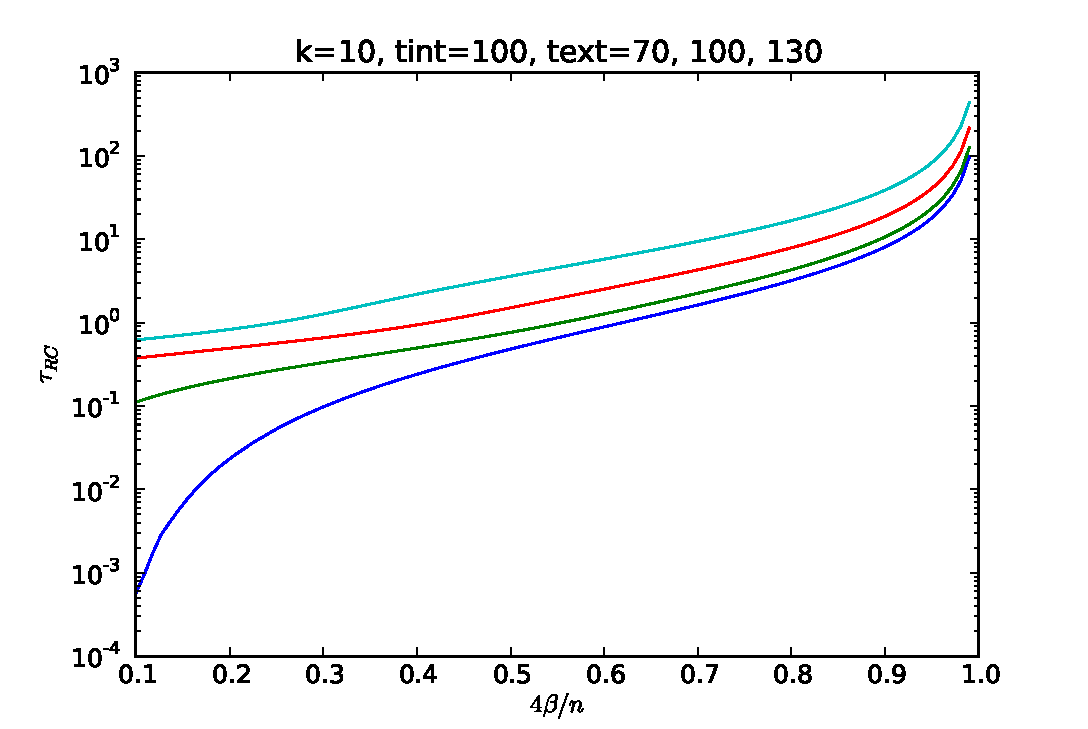
\includegraphics[width=0.45\textwidth]{taurc-vs-text-high}
  \hfill
  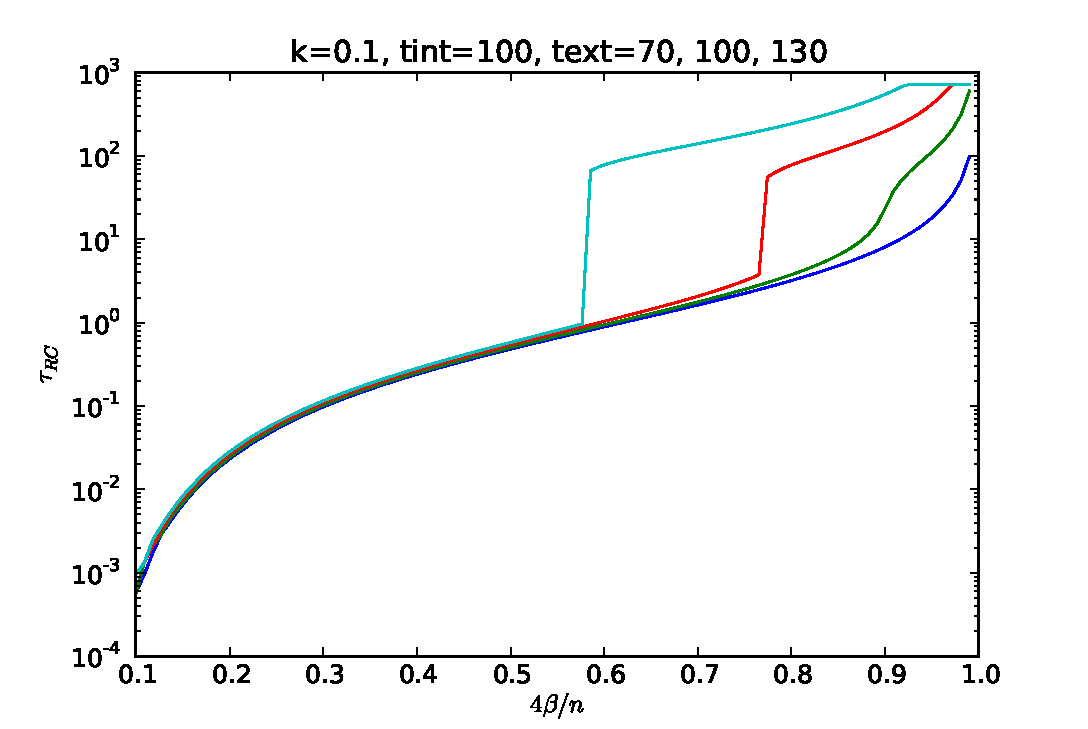
\includegraphics[width=0.45\textwidth]{taurc-vs-text-low}
  \caption{Left, optical depth of radiative/convective boundary for a
    single channel of stellar irradiation, deposited high in the
    atmosphere ($\tau\simeq 0.1$).  The x axis, characterizes the
    temperature profile of the atmosphere, with shallow profiles on
    near zero and steep profiles near 1.  On the right, the optical
    depth of the radiative-convective boundary for the case where the
    stellar irradiation is deposited low in the atmosphere.  The jumps
    in the value of $\tau_{rc}$ indication places where a deep
    radiative layer is formed.}
  \label{fig:detached-radiative-zones}
\end{figure*}

\begin{figure*}
  \centering
  % from plot_1chan_2d() in structure/python/rc.py
  \includegraphics[width=0.49\textwidth]{\string~/Dropbox/GregDave/paper1_planet_evolution/plots/10/09/fbon-flux-contour-low}
  \hfill
  \includegraphics[width=0.49\textwidth]{\string~/Dropbox/GregDave/paper1_planet_evolution/plots/10/09/fbon-flux-contour-high}
  \caption{Contours of radiative/convective boundary vs. structure of
    atmosphere (along the x axis) and ratio of external flux to
    internal flux (y axis).  On the left, depositing energy low in
    the atmosphere, on the right, depositing energy high.  The
    behavior is relatively smooth when depositing energy high in the
    atmosphere.  A discontinuity develops when depositing energy low
    in the atmosphere, and a fixed amount of energy has a larger
    effect.  }
  \label{fig:atmosphere-vs-flux}
\end{figure*}

Figure \ref{fig:atmosphere-vs-flux} shows the dependence on the
optical depth of the radiative convective transition on the structure
of the atmosphere (along the x axis) and the ratio of external flux to
internal flux for two cases, where one deposits the energy high in the
atmosphere and low in the atmosphere.  

\begin{figure}
  \centering
  % from plot_1chan_2d() in structure/python/rc.py
  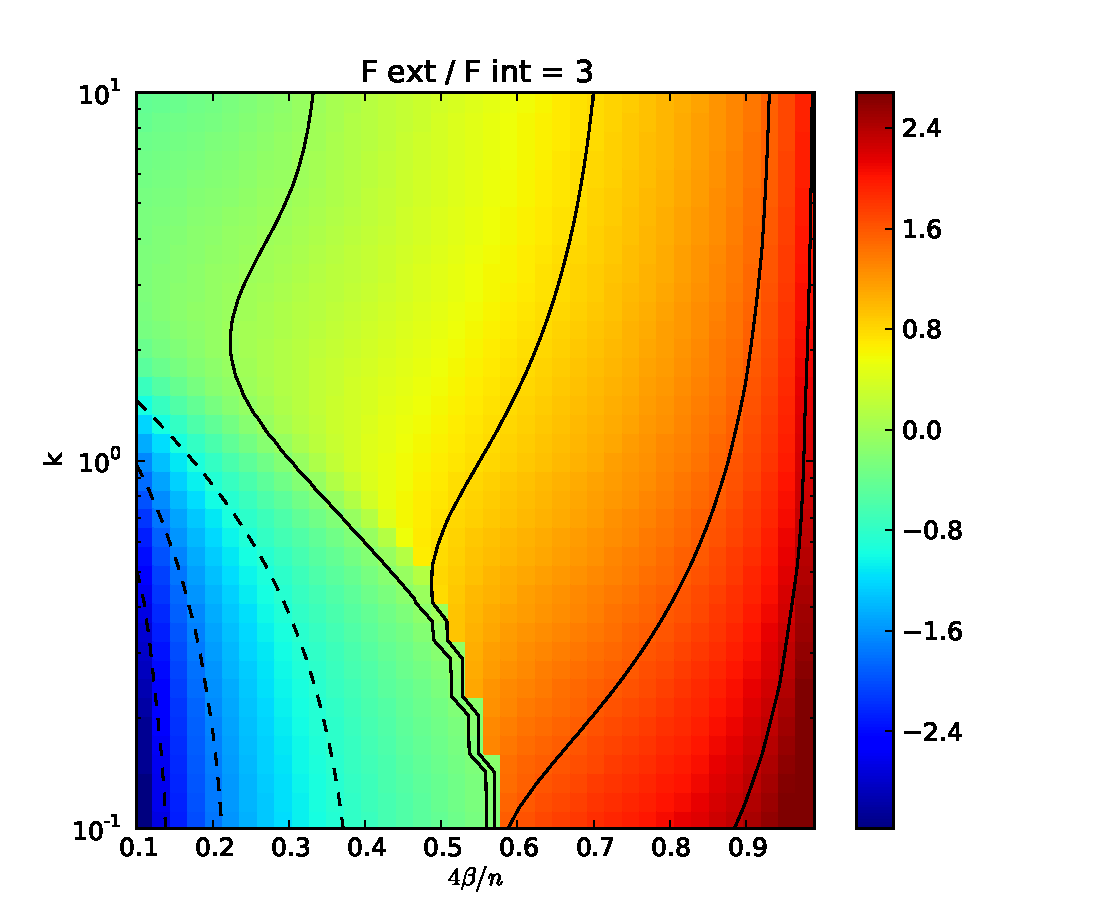
\includegraphics[width=1.0\columnwidth]{\string~/Dropbox/GregDave/paper1_planet_evolution/plots/10/09/fbon-k-contour}
  \caption{If we hold the ratio of external flux to internal flux
    constant and ask what happens to the rad/conv boundary as the
    structure of the atmosphere (x axis) and depth of energy deposit
    (y axis, high is high, low is low), then we can see the ``fold''
    develop as the energy is deposited deeper and deeper in the
    atmosphere.}
  \label{fig:atmosphere-vs-depth}
\end{figure}

Figure \ref{fig:atmosphere-vs-depth} shows what happens to the optical
depth of the rad/conv boundary if you hold the ratio of external to
internal flux fixed and vary the atmosphere (x axis) and depth of
energy deposit (y axis).  

\begin{figure*}
  \centering
% from plot_1chan_2d() in structure/python/rc.py
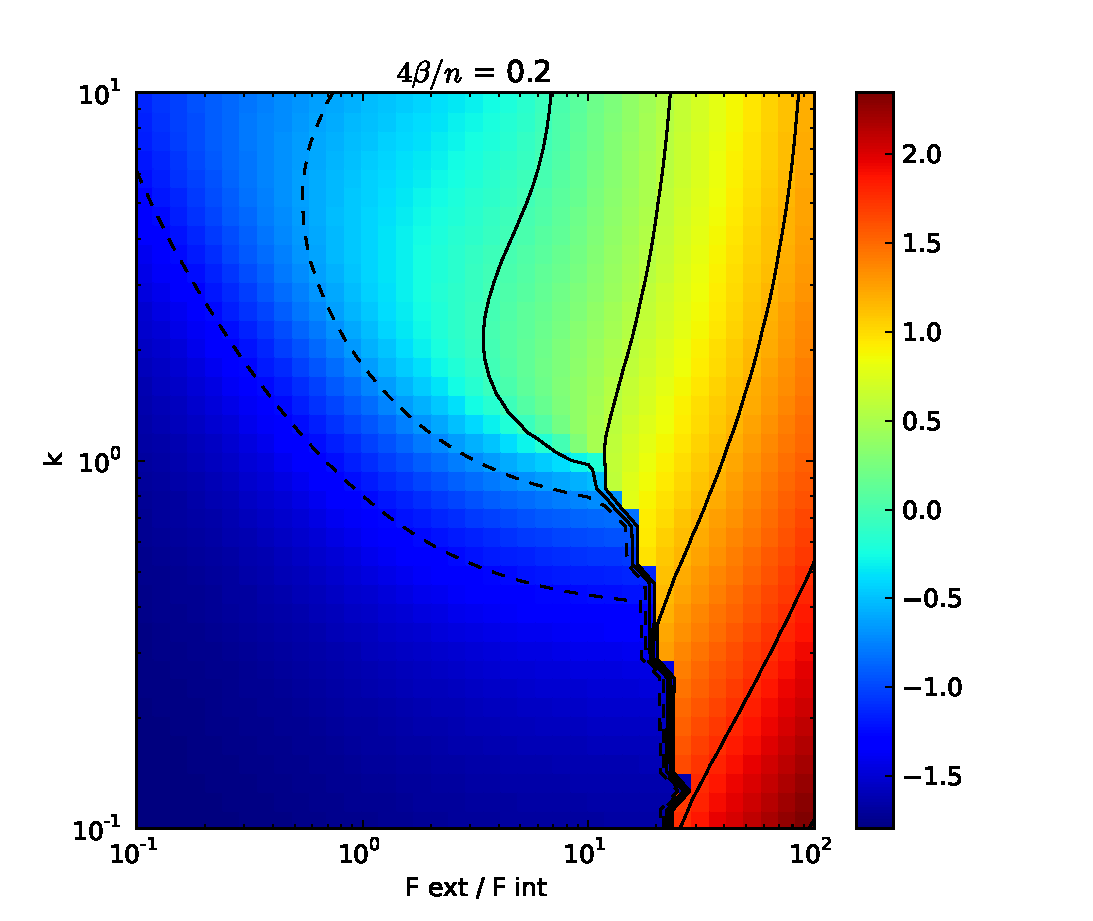
\includegraphics[width=0.32\textwidth]{\string~/Dropbox/GregDave/paper1_planet_evolution/plots/10/09/flux-k-contour-fbon-0p2}
\hfill
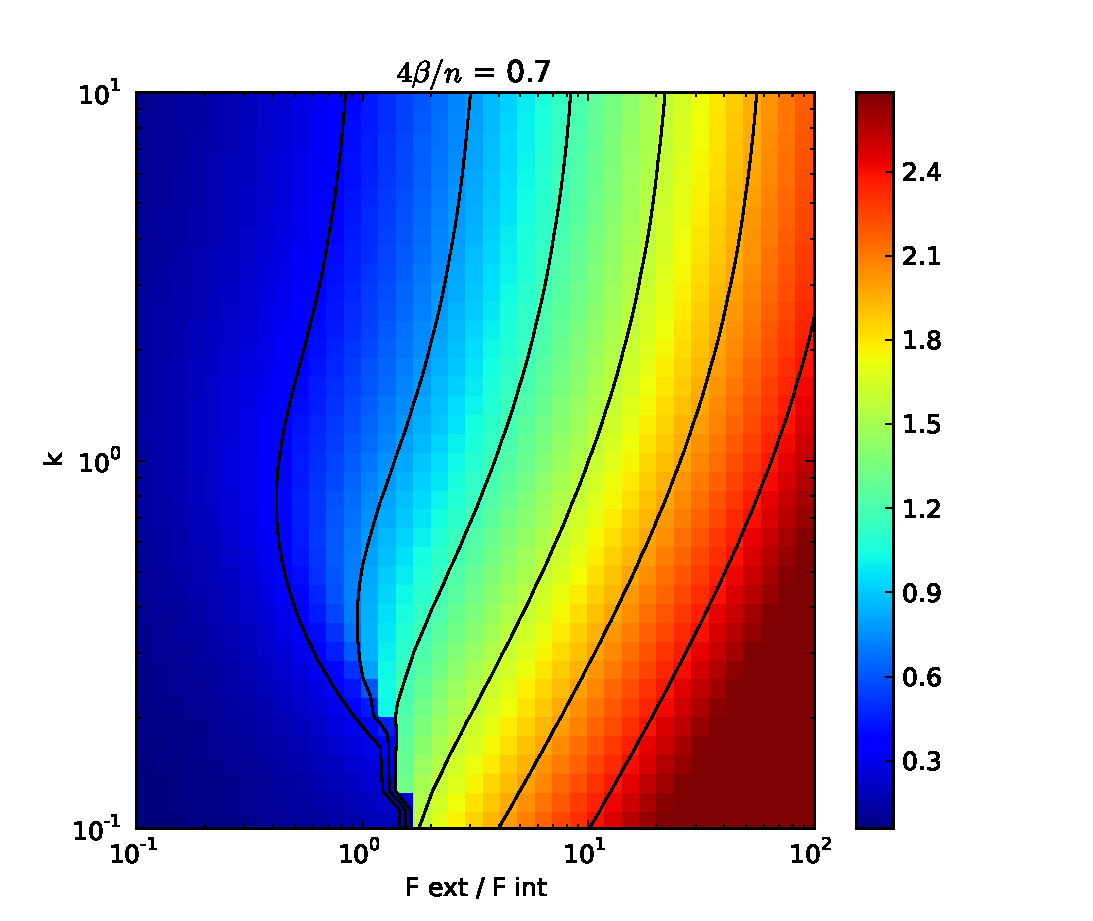
\includegraphics[width=0.32\textwidth]{\string~/Dropbox/GregDave/paper1_planet_evolution/plots/10/09/flux-k-contour-fbon-0p7}
\hfill
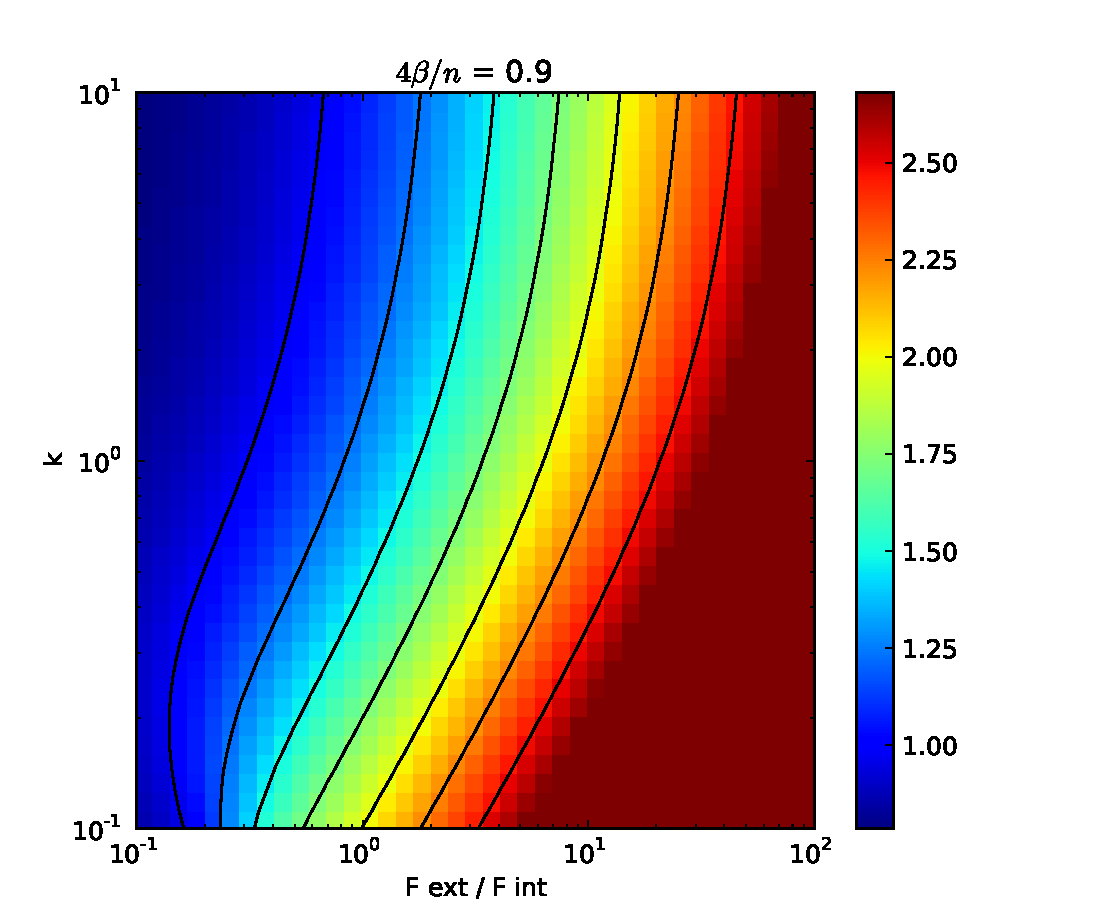
\includegraphics[width=0.32\textwidth]{\string~/Dropbox/GregDave/paper1_planet_evolution/plots/10/09/flux-k-contour-fbon-0p9}
\caption{Optical depth of the rad/conv transition for three different
  atmosphere structures, from shallow temp profile (left) to steep
  temp profile (right).  The x axis gives the ratio of external flux
  to internal flux (small ratio on the left, large ratio on the right)
  while the y axis gives the depth at which the energy is deposited
  (low for low, high for high).  One sees that depositing the energy
  deeper has a larger effect, and a ``fold'' structure develops for
  atmospheres with shallow temperature profiles.}
\label{fig:flux-vs-depth}
\end{figure*}

Figure \ref{fig:flux-vs-depth} shows what happens to the optical depth
of the rad/conv boundary as a function of external to internal flux
ratio and depth of energy deposit.  

\begin{figure*}
% from plot_grav_1chan() in structure/python/rc.py
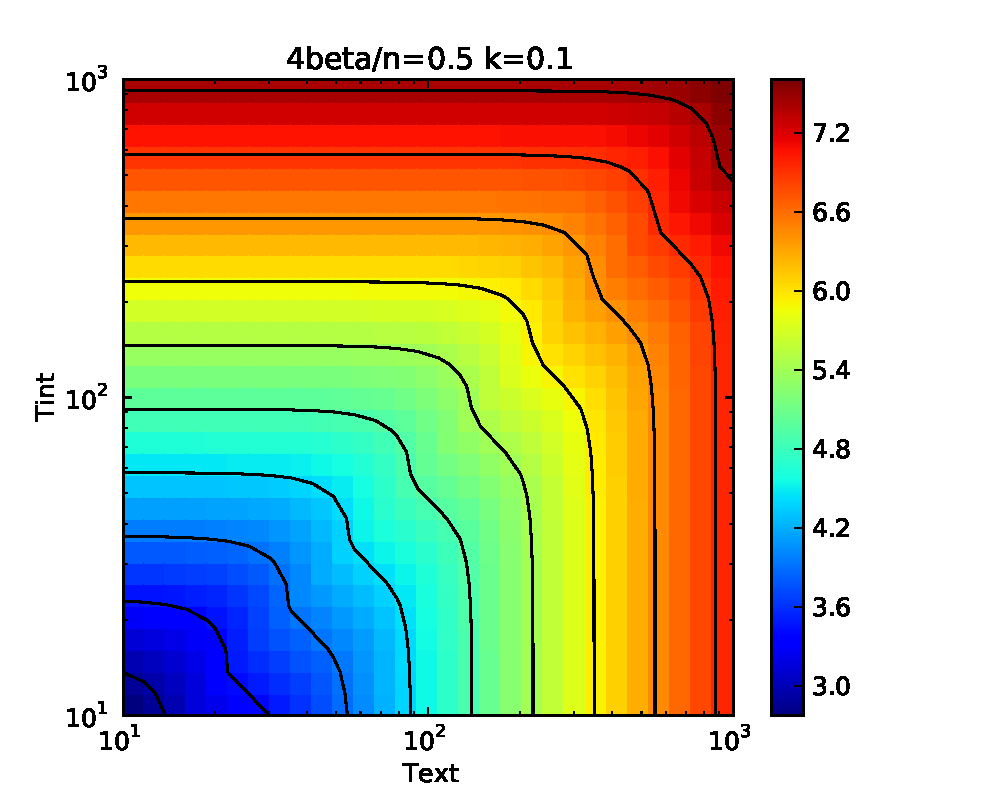
\includegraphics[width=0.45\textwidth]{\string~/Dropbox/GregDave/paper1_planet_evolution/plots/10/09/grav-1chan-fbon-0p5-k-0p1}
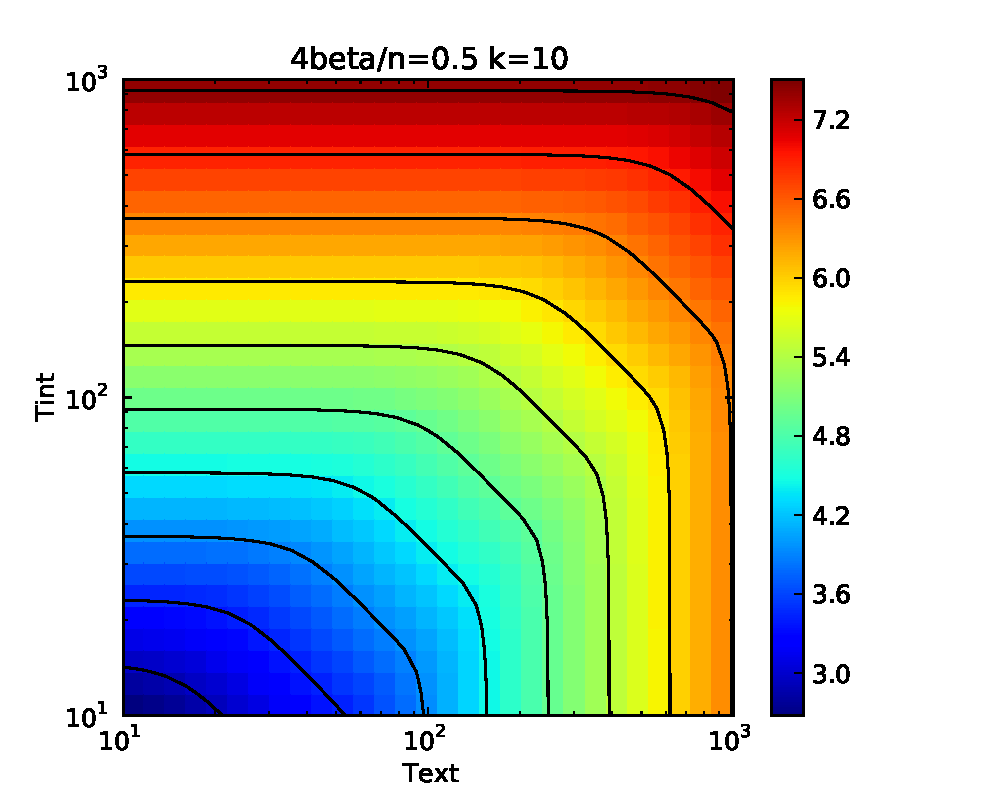
\includegraphics[width=0.45\textwidth]{\string~/Dropbox/GregDave/paper1_planet_evolution/plots/10/09/grav-1chan-fbon-0p5-k-10}
\caption{Contours of surface gravity as a function of effective
  temperature of external radiation (x axis) and effective temperature
of of planet's cooling radiation (y axis).  On the left, for energy
deposited deep in the atmosphere, on the right, high in the
atmosphere.   One can see that at fixed surface gravity (along a
contour), increasing Text causes Tint to fall in a well-defined
fashion, with somewhat interesting behavior around $Text \simeq Tint$
when depositing energy deep in the atmosphere.}
\label{fig:surf-grav-vs-text-and-tint}
\end{figure*}

Figure \ref{fig:surf-grav-vs-text-and-tint} shows what happens to the
internal flux as you change the irradiation temperature for fixed
surface gravity.  At low Text, the internal temp is whatever it will
be, and then as the external flux increases the internal flux drops.  

\begin{figure}
% from plot_grav_1chan() in structure/python/rc.py
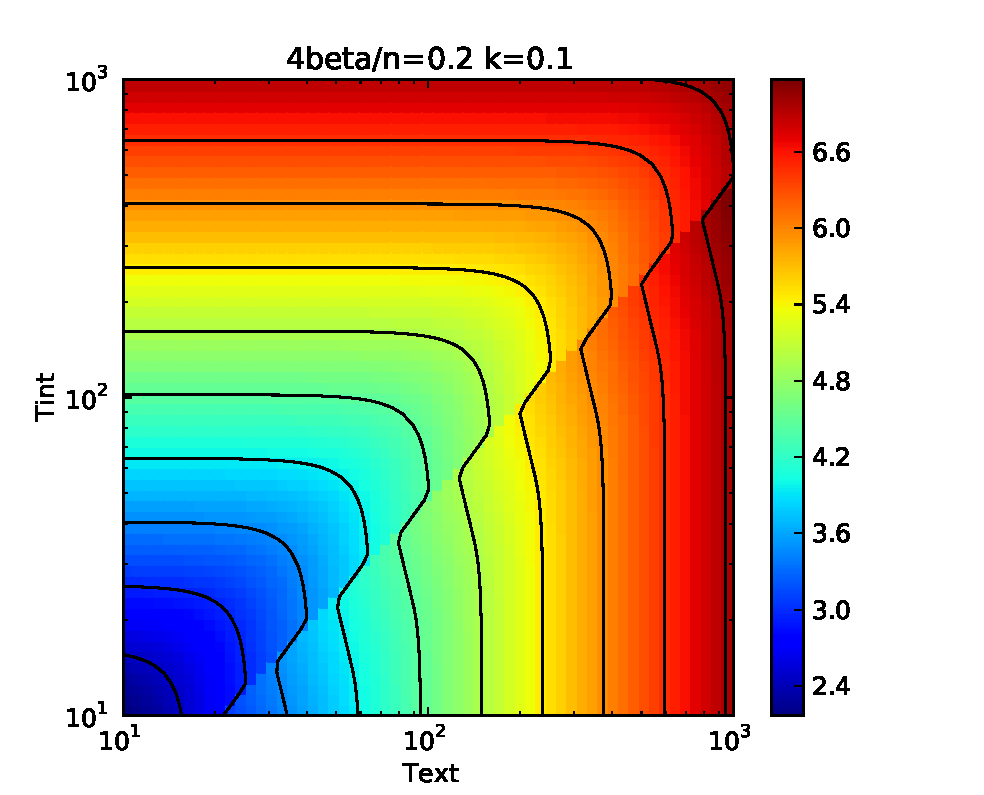
\includegraphics[width=0.45\textwidth]{\string~/Dropbox/GregDave/paper1_planet_evolution/plots/10/09/grav-1chan-fbon-0p2-k-0p1}
\caption{Contours of surface gravity as a function of effective
  temperature of external radiation (x axis) and effective temperature
  of of planet's cooling radiation (y axis), when depositing energy
  deep in the atmosphere.  The same as the previous figure, except
  that the structure of the atmosphere is different, the temperature
  profile being shallower.  One sees that the contours of surface
  gravity develop an ``overbite'' as Text approaches Tint.  This would
  indicate that for fixed surface gravity, Tint is no longer a
  single-valued function of Text.  I'm not sure what this means.  Does
  stability determine which solution is selected?}
\label{fig:surf-grav-vs-text-and-tint-shallow-temp-profile}
\end{figure}

Figure \ref{fig:surf-grav-vs-text-and-tint-shallow-temp-profile} shows
the same thing as the previous figure, except that the overall
temperature profile is shallower and Tint as a function of Text at
fixed surface gravity becomes double-values for certain choices of
Text.  It is not clear to me what this means.  

\subsubsection{Via Tables}

An atmospheric boundary condition can be provided via any function
that takes surface gravity and bulk entropy of the planet and computes
the luminosity.  This can be via a table lookup for such a table
computed by a program such as TLUSTY.

\section{Maximum Entropy of Solutions}

I find myself thinking again about the maximum entropy of solutions of
finite radius.  If the entire solution is on an adiabat, what can I
say about that solution?  Consider first the usual case where
electrons are fully degenerate and provide pressure while protons are
non-degenerate and provide entropy.  

EOS:
\begin{equation}
  P = \frac{\hbar}{m_e} n^{5/3}
\end{equation}
HSE:
\begin{equation}
  P_c = \frac{G M^2}{R^4}
\end{equation}
together:
\begin{equation}
  R = \frac{\hbar^2}{m_e m_p^{5/3} G M^{1/3}}
\end{equation}
which gives
\begin{equation}
  P_c = \frac{G^5 M^{10/3} m_e^4 m_p^{20/3}}{\hbar^8}
\end{equation}
I can also get the escape velocity of the planet
\begin{equation}
  v_{esc} = \frac{G M^{2/3} m_e^{1/2} m_p^{5/6}}{\hbar}
\end{equation}
Now I know that $T\propto n^{2/3}$ for an adiabat.  More specifically
\begin{equation}
  \psi = \log \frac{n}{n_{q,e}} = \log \left(\frac{T}{T_F}\right)^{-3/2}
\end{equation}
\begin{equation}
  n = n_{q,e} e^\psi
\end{equation}
then
\begin{equation}
  n = \left(\frac{m_e k T}{\hbar^2}\right)^{3/2} e^\psi
\end{equation}
and
\begin{equation}
  kT = \frac{\hbar^2}{m_e} e^{-2\psi/3} n^{2/3}
\end{equation}
I want to know something at the surface.  Do I want to know the
thermal velocity or the Fermi velocity?  Do I want to know the
velocity of the electrons or the protons?  It's not clear to me.
\begin{equation}
  v_{Fe} = \sqrt{\frac{k T_F}{m_e}} = \frac{\hbar n^{1/3}}{m_e}
\end{equation}
\begin{equation}
  v_{te} = \sqrt{\frac{k T}{m_e}}
\end{equation}
\begin{equation}
  v_{tp} = \sqrt{\frac{k T}{m_p}}
\end{equation}

Now I would like estimates of the density and temperature at the
surface.  One definition of the surface is $P=0$ but that gives $\rho
= T = 0$.  I want the point where the $T$ profile goes off of an
adiabat.  This will happen at least above the $\tau=1$ surface,
perhaps deeper.  Let's say that it happens at $N$ optical depths.
\begin{equation}
  \delta R = \frac{N}{\rho \kappa}
\end{equation}
and HSE gives
\begin{equation}
  \frac{P_s - 0}{\delta R} = \frac{G M \rho}{R^2}
\end{equation}
so 
\begin{equation}
  P_s = \frac{G M N}{\kappa R^2} 
  = \frac{N g}{\kappa} 
  = \frac{G^3M^{5/3} N m_e^2 m_p^{10/3}}{\kappa \hbar^4}
\end{equation}
which gives the surface number density
\begin{equation}
  n_s = \frac{G^{9/5} M N^{3/5} m_e^{9/5} m_p^2}{\kappa^{3/5} \hbar^{18/5}}
\end{equation}
and the surface temperature
\begin{equation}
  k T_s = \frac{e^{-2\psi/3} G^{6/5} M^{2/3} N^{2/3} m_e^{1/5} m_p^{4/3}}{\kappa^{2/5}\hbar^{2/5}}
\end{equation}

These allow me to write the velocities at the surface.  Repeating the
escape velocity and putting in the surface temperature/density for the others:
\begin{equation}
  v_{esc} = \frac{G M^{2/3} m_e^{1/2} m_p^{5/6}}{\hbar}
\end{equation}
(note that this looks like a ratio involving the Chandra mass)
\begin{equation}
  v_{Fe} = \frac{G^{3/5} M^{1/3} N^{1/5} m_p^{2/3}}
  {\kappa^{1/5} \hbar^{1/5} m_e^{2/5}}
\end{equation}

\begin{equation}
  v_{te} = \frac{e^{-\psi/3}G^{3/5} M^{1/3} N^{1/5} m_p^{2/3}}
  {\kappa^{1/5} \hbar^{1/5} m_e^{2/5}}
\end{equation}

\begin{equation}
  v_{tp} = \frac{e^{-\psi/3}G^{3/5} M^{1/3} N^{1/5} m_p^{1/6} m_e^{1/10}}
  {\kappa^{1/5} \hbar^{1/5}}
\end{equation}

So $v_{te}$ is the same as $v_{Fe}$ suppressed by the degeneracy
prameter, and $v_{tp}$ is the same as $v_{te}$, suppressed by the
square root of the electron proton mass ratio.  But the escape
velocity scales differently.  Form the ratio
\begin{equation}
  \frac{v_{Fe}}{v_{esc}} = \frac{N^{1/5} \hbar^{4/5}}{\kappa^{1/5}
    G^{2/5} M^{1/3} m_e^{1/2} m_p^{1/6}}
\end{equation}
This is $6 \times 10^{-11}$ for a Jupiter mass, or unity for 0.4
grams.  That is to say that all relevant velocities are much less than
the escape velocity.

\subsection{Lane-Emden Equation}
Taking the solutions of the Lane-Emden equation and putting the
dimensional parts back in, we have:

\begin{equation}
  % K+W 19.3
  P = K \rho ^\gamma = K \rho^{1+\frac{1}{n}}
\end{equation}
\begin{equation}
  % K+W 19.9
  R = \frac{z_n}{A}  
\end{equation}
\begin{equation}
  A = \sqrt{\frac{4\pi G}{(n+1) K}}\rho_c^{\frac{n-1}{2n}}
\end{equation}
\begin{equation}
  %K+W 19.20
  \rho_c = \frac{M z_n^3}{4\pi R^3 D_n}
\end{equation}
\begin{equation}
  % Take value from Table 19.1
  D_n = \left( -z^2 \frac{dw}{dz}\right)_{z=z_n}
\end{equation}
where $w$ and $z$ are the dimensionless variables in which the LE
equation is written, $z_n$ is the value of $z$ where $w=0$ (the
surface of the object)

Then we may finally write 
\begin{equation}
  R = z_n 
  M^{\frac{1-n}{3-n}}
  (n+1)^{\frac{n}{3-n}}
  K^{\frac{n}{3-n}}
  (4 \pi D_n)^{\frac{n-1}{3-n}}
  (4 \pi G)^{\frac{n}{n-3}}
\end{equation}

Now what is $K$?  Dispense with all unitless coefficient of order
unity, but keep everything that appears in an exponent.  It's always
the case that protons provide the entropy (thus fix the temperature)
and electrons provide the pressure.  I want to write the EOS in terms
of density and entropy.  Consider three cases in turn.  First, protons
and electrons are both degenerate (so that the entropy is given above,
and is not the Sakur-Tetrode equation).  Then
\begin{equation}
  P = \frac{\hbar^2}{m_e m_p^{5/3}} \left( 1+\frac{kT}{kT_F} \right) \rho^{5/3} 
\end{equation}
with 
\begin{equation}
  k T_F = \frac{\hbar^2 n^{2/3}}{m_e}
\end{equation}
and 
\begin{equation}
  kT = \frac{\hbar^2 n^{2/3} \sigma}{m_p}
\end{equation}
so 
\begin{equation}
  P = \frac{\hbar^2}{m_e m_p^{5/3}}
\left(1 + \frac{m_e \sigma}{m_p} \right)
\rho^{5/3}
\end{equation}
which is valid for $\sigma < 1$

Second case: electrons degenerate, protons non-degenerate.  Then the
Sakur-Tetrode equation gives
\begin{equation}
  kT = \frac{\hbar^2}{m_p} n^{2/3} 
\exp\left(\frac{2\sigma}{3} - \frac{5}{3}\right)
\end{equation}
and the EOS is
\begin{equation}
  P = \frac{\hbar^2}{m_e m_p^{5/3}}
\left[1 + \frac{m_e}{m_p} 
\exp\left(\frac{2\sigma}{3} - \frac{5}{3}\right) \right]
\rho^{5/3}
\end{equation}
which is valid for $1 < \sigma < 11$

Third case: electrons and protons non-degenerate.  The relation
between entropy and temperature is the same, so the EOS gives.
\begin{equation}
  P = \frac{\hbar^2}{m_p^{8/3}} 
\exp\left(\frac{2\sigma}{3} - \frac{5}{3}\right) 
\rho^{5/3}
\end{equation}
which is valid for $11 < \sigma$.

\section{Conclusions}
\label{sec:conc}

\acknowledgements

%We thank NO ONE.  We did it BY OURSELVES.  With NO HELP.  From ANYONE.

\bibliography{biblio}

\clearpage

\end{document}
